\chapter{Popis vstupných dát a ich spracovanie}
\label{chap:ThirdChapter}
\section{Charakteristika vstupných PDF dokumentov}
\subsection{Typy PDF dokumentov}
\begin{hyphenrules}{nohyphenation}
Ako už bolo spomenuté v predchádzajúcej kapitole, typy PDF dokumentov, ktorým sa v práci venujeme, sú dva; prvým typom sú skenované fyzické originály dokumentov, druhým sú digitálne dokumenty. Zásadným rozdielom je šum pri skenovaných dokumentoch, ktorý sa v digitálnych dokumentoch nenachádza. Môže sa napríklad jednať o nedokonalosti spôsobené nesprávnym priložením papierovej predlohy na skener (obr.  \ref{fig:3.1} vľavo). Vpravo je ukážka digitálnej zmluvy.

\begin{figure}[H]
\begin{minipage}[t]{.35\linewidth}
\fbox{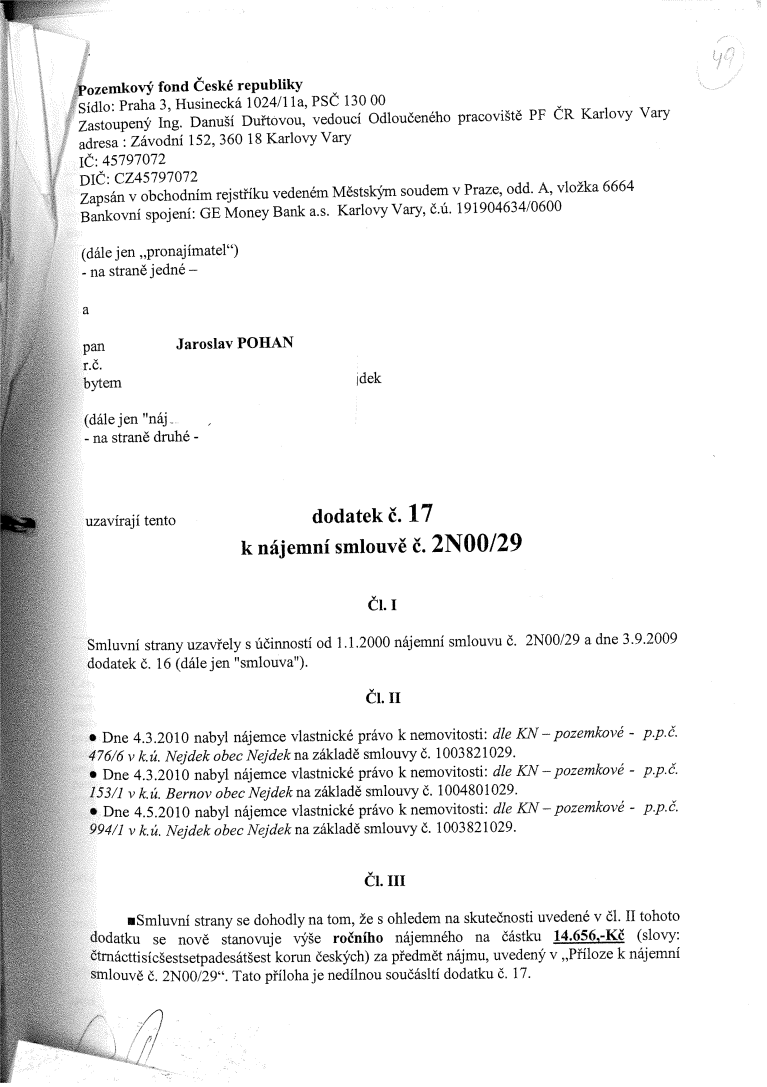
\includegraphics[width=0.9\linewidth]{img/577.png} }
\end{minipage}\hfill
\begin{minipage}[b]{.35\linewidth}
\fbox{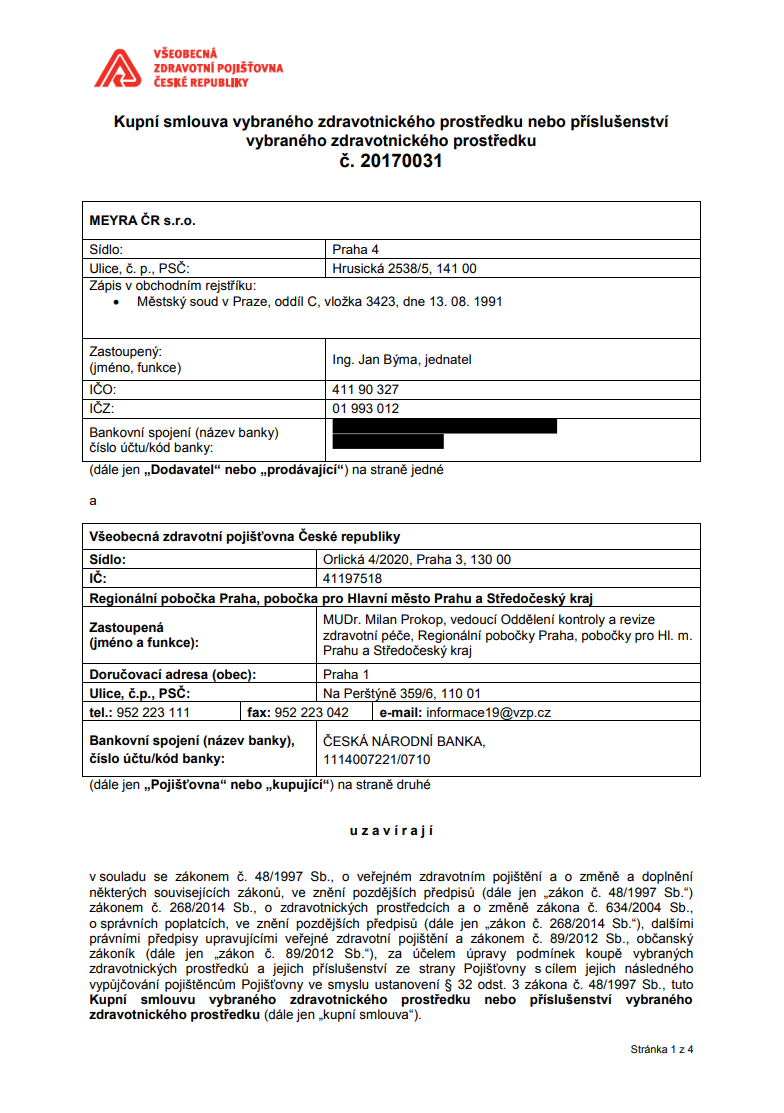
\includegraphics[width=0.9\linewidth]{img/2736.png}}
\end{minipage}
\caption{Porovnanie rozdielu medzi skenovaným (vľavo) a digitálnym dokumentom (vpravo).}
\label{fig:3.1} 
\end{figure}

K analýze vstupných dát sme si pripravili jednoduchý program (obr. \ref{fig:3.2}) (viac v podkapitole \ref{chap:6.3.1}), ktorý priebežne z desaťtisíc odkazov na stiahnutie zmlúv, ktoré nám boli na vyžiadanie zaslané z portálu \url{https://smlouvy.gov.cz}\cite{smlouvy-gov}, sťahoval dokumenty a zobrazoval jednotlivé stránky. 

\begin{figure}[H]
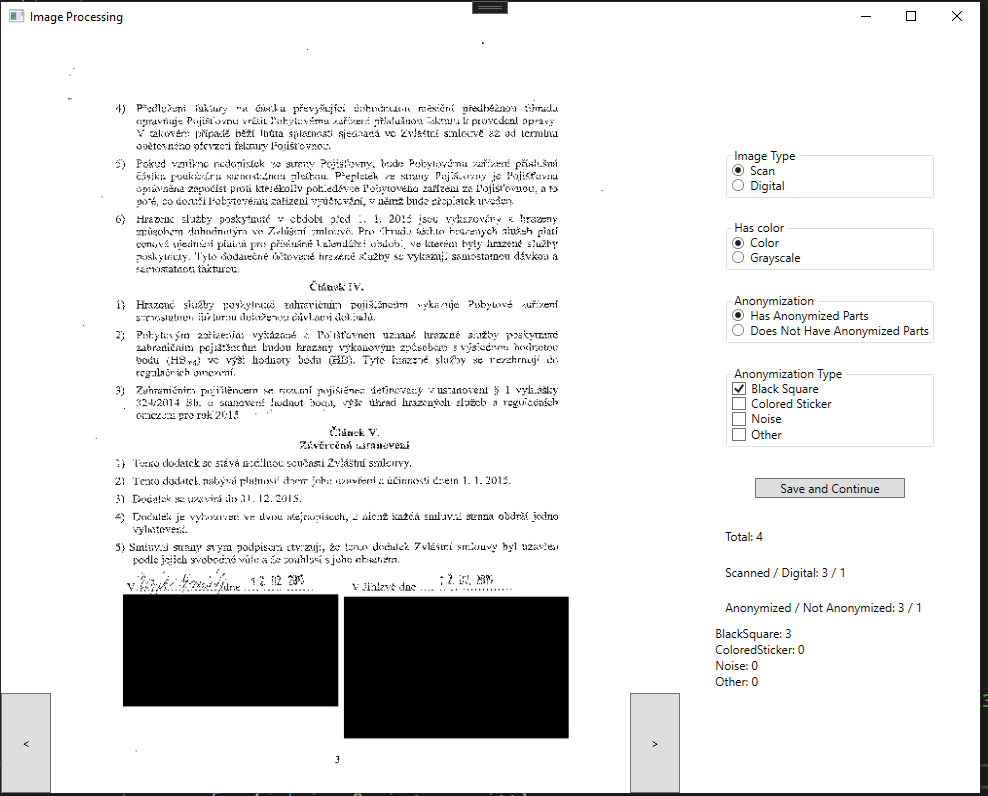
\includegraphics[width=\linewidth]{img/image_proc.png}
\caption{Grafické rozhranie skriptu \texttt{ManualCheckerUtility} (\ref{chap:6.3.1}).}
\label{fig:3.2}
\end{figure}

Následne sme pomocou tejto aplikácie vytvorili štatistiku nad týmito dokumentmi, kde sme zistili nasledovné:

\floatsetup[table]{capposition=top}
\begin{table}[H]
\caption{Štatistika nad manuálne skúmanými PDF dokumentmi.}
\label{table:3.1}
\begin{tabular}{|l|c|}
\hline
\textbf{Celkový počet:} & 161 \\ \hline
\textbf{Sken / Digitál :} & 129 / 32 \\ \hline
\textbf{Anonymizované / Neanonymizované:} & 122 / 39 \\ \hline
\textbf{Čierny obdĺžnik:} & 118 \\ \hline
\textbf{Farebná nálepka:} & 1 \\ \hline
\textbf{Šum:} & 2 \\ \hline
\textbf{Ostatné:} & 1 \\ \hline
\end{tabular}
\end{table}
Príklady typov anonymizácií, ktoré sme manuálnym prehľadávaním našli:

\begin{table}[H]
\centering
\caption{Typy anonymizácií, ktoré sme manuálnym prehľadávaním našli.}
\label{table:3.2}
\begin{tabular}{|c|c|}
\hline
\textbf{Typ} & \textbf{Obrázok} \\ \hline
Šum & 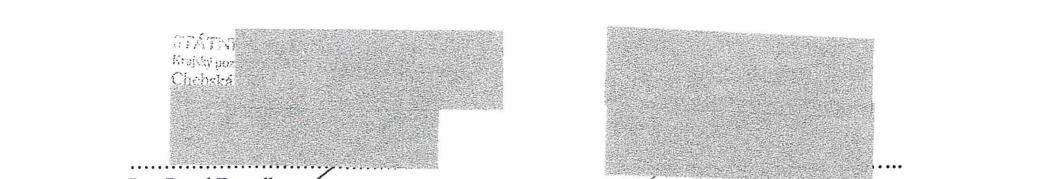
\includegraphics[width=0.5\linewidth]{img/2577_sum.png} \\ \hline
Čierny obdĺžnik & 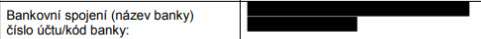
\includegraphics[width=0.5\linewidth]{img/2736_sum.png} \\ \hline
Ostatné & 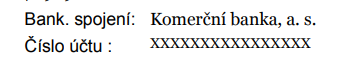
\includegraphics[width=0.5\linewidth]{img/4756_sum.png} \\ \hline
Farebná nálepka & 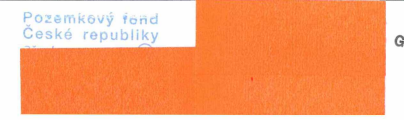
\includegraphics[width=0.5\linewidth]{img/798_sum.png} \\ \hline
\end{tabular}
\end{table}


\subsection{Typické anonymizované oblasti}
Vzhľadom na to, že dokumenty pred anonymizáciou nie sú dostupné, môžeme len s pravdepodobnosťou na základe logického uváženia určovať, čo bolo predmetom anonymizovania. Zväčša sa jednalo o začiernenie podpisov, mien (obr. \ref{fig:3.3} vľavo) a rodných čísel, vzhľadom na kontext okolitého textu sa vyskytlo niekoľkokrát aj zamazanie názvov firiem, čísel účtov či súm, ak sa jednalo o kúpne či predajné zmluvy a v niekoľkých špecifických prípadoch boli prekryté čiernym štvorcom celé strany, takže nebolo možné identifikovať ani to, čo bolo obsahom, resp. predmetom zmluvy (obr. \ref{fig:3.3} vpravo). 

\begin{figure}[H]
\begin{minipage}[t]{.3\linewidth}
\fbox{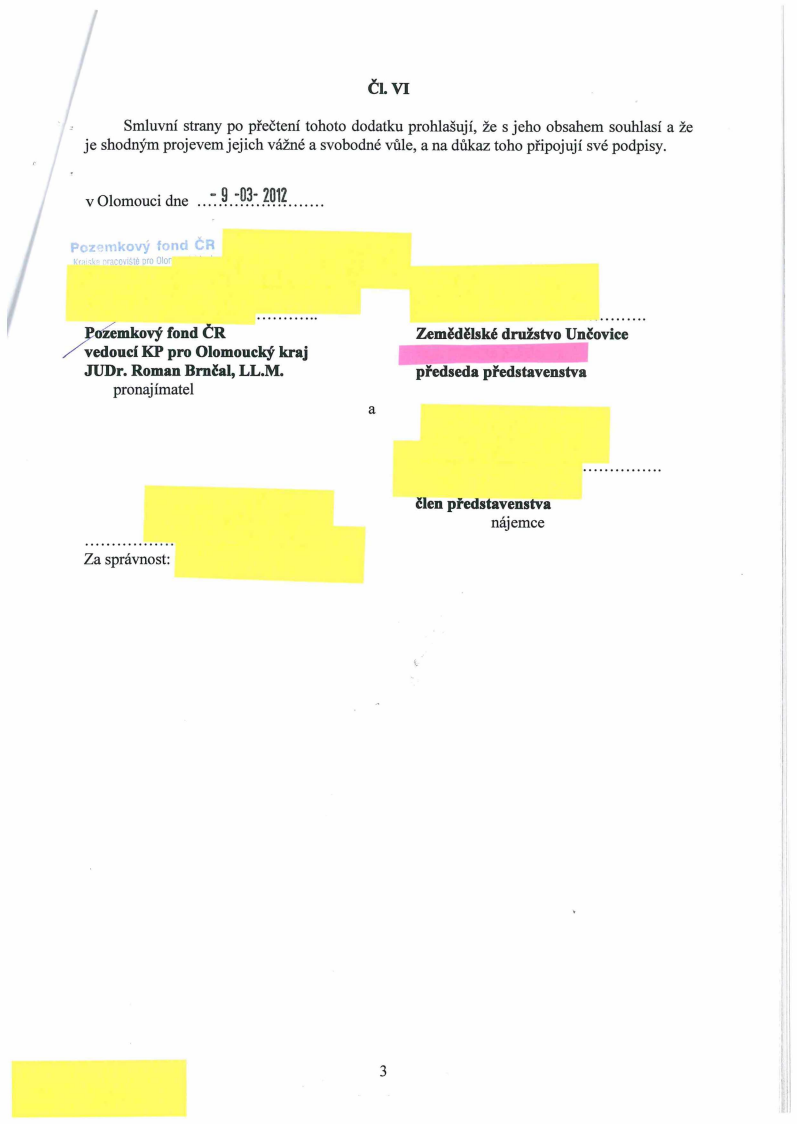
\includegraphics[width=0.8\linewidth]{img/4280.png}}
\caption{Príklady anonymizovaných oblastí, vľavo bežný výskyt, vpravo výskyt, kde bola začiernená celá strana.}
\label{fig:3.3} 
\end{minipage}\hfill
\begin{minipage}[b]{.3\linewidth}
\fbox{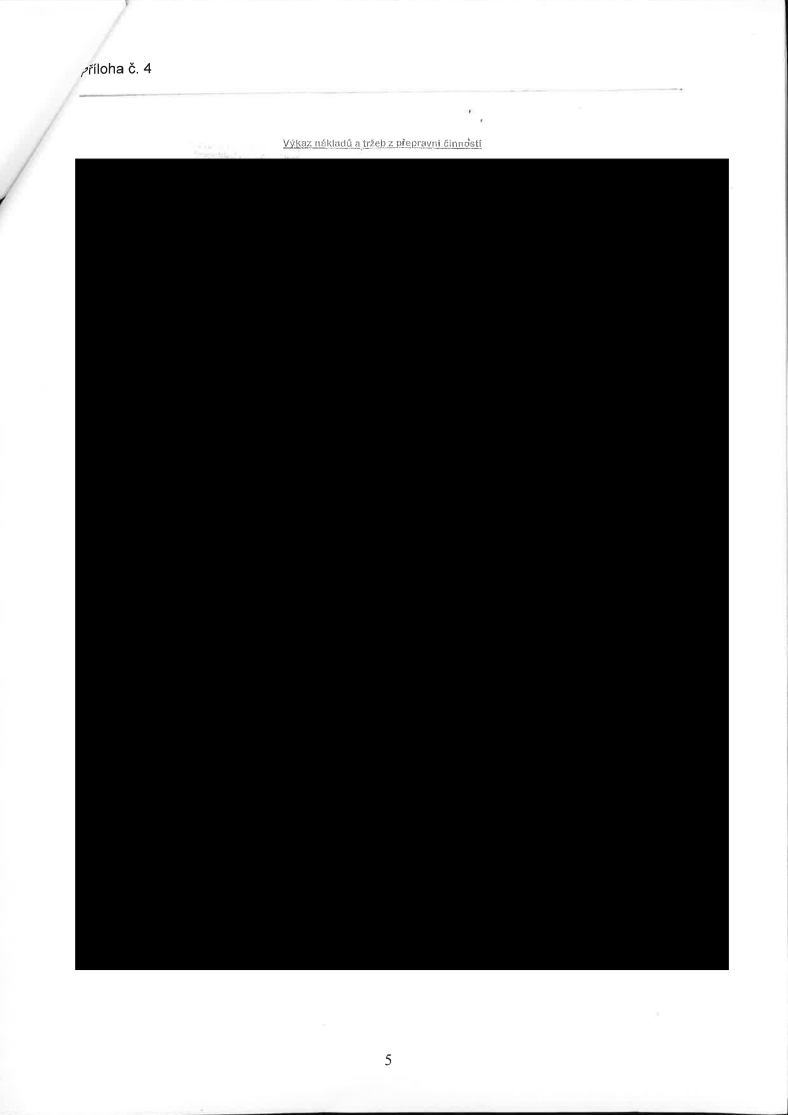
\includegraphics[width=0.8\linewidth]{img/4132.png}}
\end{minipage}
\end{figure}

Keďže len zhruba 25 \% dokumentov, nad ktorými sme urobili štatistiku, obsahovalo anonymizované dáta, usudzujeme, že tieto údaje sú najčastejšími údajmi, ktoré sú anonymizované.
\newline

Vzhľadom na prístup k detekcii anonymizovaných oblastí sa nebudeme zaoberať detekciou typu "Ostatné" znázornenej v tabuľke \ref{table:3.2}.
\section{Predspracovanie dát}
\subsection{Predpríprava dokumentov}
Keďže jednotlivé dokumenty spravidla obsahujú viac strán, je nutné analyzovať každú stranu. Z tohoto dôvodu sme sa rozhodli zo vstupných PDF dokumentov vytvárať obrázky jednotlivých strán pomocou knižnice \texttt{MagickImage} a ukladať ich ako \texttt{byte[]}. Týmto rozhodnutím síce prídeme o informácie a metadata z~digitálnych originálov PDF dokumentov, každopádne vzhľadom na to, že majorita dokumentov (tabuľka \ref{table:3.1}) sú skeny a typ anonymizácie je spravidla čierny obdĺžnik (tabuľka \ref{table:3.1}, ktorý je relatívne jednoducho detegovaný, je jednoduchšie pracovať s jedným formátom dokumentu, a to vo forme obrázku jednotlivej strany. Tento formát je pre nás najjednoduchší na spracovanie pomocou algoritmov počítačového videnia. 
\newline

Obrázky sme ďalej needitovali, pre ďalšie spracovanie sme použili obrázky o~veľkosti približne 850x600 pixelov (čo zodpovedá rozmerom štandardného papiera ISO A\cite{prepressure}), resp. 600x850 pixelov ak sa jednalo o formát na šírku.

\subsection{Výzvy a riešenia}
Jednou z výziev pri analýze dokumentov je rôznorodá kvalita skenov. S týmto sa spája viac problémov, ktoré môžu nastať, zväčša sa jedná o spomínaný šum, ktorý vznikne nedokonalým priložením predlohy na skener. Problém so šumom sme riešili pomocou filtračných techník na zníženie šumu v obrázkoch.
\newline

Ďalším z problémov je zarovnanie strany. Pri skenovaní sa môže stať, že výsledný sken nebude zarovnaný. Orientácia strany je dôležitá pri výpočte pomeru anonymizovaných oblastí vzhľadom k celej strane dokumentu. Orientáciu strán sme v našom algoritme ani v predpríprave dokumentov neriešili, nakoľko všetky testované dokumenty boli spravidla zarovnané a len v pár prípadoch boli skeny vychýlené natoľko, že by to mohlo závažne ovplyvniť výsledné percento. 
\end{hyphenrules}
